%%%%%%%%%%%%%%%%%%%%%%%%%%%%%%%%%%%%%%%%%
% Thin Sectioned Essay
% LaTeX Template
% Version 1.0 (3/8/13)
%
% This template has been downloaded from:
% http://www.LaTeXTemplates.com
%
% Original Author:
% Nicolas Diaz (nsdiaz@uc.cl) with extensive modifications by:
% Vel (vel@latextemplates.com)
%
% License:
% CC BY-NC-SA 3.0 (http://creativecommons.org/licenses/by-nc-sa/3.0/)
%
%%%%%%%%%%%%%%%%%%%%%%%%%%%%%%%%%%%%%%%%%

%----------------------------------------------------------------------------------------
%	PACKAGES AND OTHER DOCUMENT CONFIGURATIONS
%----------------------------------------------------------------------------------------

\documentclass[letterpaper,10pt]{article} % Font size (can be 10pt, 11pt or 12pt) and paper size (remove a4paper for US letter paper)
\usepackage[margin=1.6in]{geometry}
\usepackage[protrusion=true,expansion=true]{microtype} % Better typography
\usepackage{graphicx} % Required for including pictures
\usepackage{caption}
\usepackage{subcaption}
\usepackage{wrapfig} % Allows in-line images

\usepackage{mathpazo} % Use the Palatino font
\usepackage[T1]{fontenc} % Required for accented characters
\linespread{1.05} % Change line spacing here, Palatino benefits from a slight increase by default

\makeatletter
\renewcommand\@biblabel[1]{\textbf{#1.}} % Change the square brackets for each bibliography item from '[1]' to '1.'
\renewcommand{\@listI}{\itemsep=0pt} % Reduce the space between items in the itemize and enumerate environments and the bibliography

\newcommand{\ffig}[3]{
\begin{figure}[h!]
\centering
\includegraphics[width=0.8\textwidth]{#1}
\caption{#2}
\label{fig:#3}
\end{figure}
}

\renewcommand{\maketitle}{ % Customize the title - do not edit title and author name here, see the TITLE block below
\begin{flushright} % Right align
{\LARGE\@title} % Increase the font size of the title

\vspace{5pt} % Some vertical space between the title and author name

{\large\@author} % Author name
\vspace{0pt} % Some vertical space between the author block and abstract
\end{flushright}
}

%----------------------------------------------------------------------------------------
%	TITLE
%----------------------------------------------------------------------------------------

\title{\textbf{Manipulation Algorithms Midterm Project Report}\\ % Title
Trajectory Retiming for Manipulation Planning} % Subtitle

\author{\textsc{Arjun Menon} % Author
\\{\textit{Carnegie Mellon University}}} % Institution

%----------------------------------------------------------------------------------------

\begin{document}

\maketitle % Print the title section

%----------------------------------------------------------------------------------------
%	ABSTRACT AND KEYWORDS
%----------------------------------------------------------------------------------------

%\renewcommand{\abstractname}{Summary} % Uncomment to change the name of the abstract to something else

%\begin{abstract}
%
%\end{abstract}
%
%\hspace*{3,6mm}\textit{Keywords:} lorem , ipsum , dolor , sit amet , lectus % Keywords
%
%\vspace{10pt} % Some vertical space between the abstract and first section

%----------------------------------------------------------------------------------------
%	ESSAY BODY
%----------------------------------------------------------------------------------------

\section{Proposed Planner}\label{sec:proposed}

In this project, the approach used in "Kinodynamic Planning in the Configuration Space via Velocity Interval Propagation" for kinodynamic planning is explored and extended for dealing with dynamic obstacles~\cite{pham2013velocity}. Using a modified RRT extension algorithm, they sample in configuration space and maintain with each node the reachable set of path-parametrized velocities. The reachable set of velocities allows then to keep track of possible node-to-node retimings which can then be chained together to get a whole-plan retiming. The completeness of the planner is in question however, and one of the goals for this project is to address this shortcoming by reformulating the problem as graph-search.

In the following sections, the major implementation components for the project is described starting with Bobrow's Algorithm, the Dynamic Obstacle Representation, and Prototypical Successor Generation trials.

\begin{figure}[h]
\centering
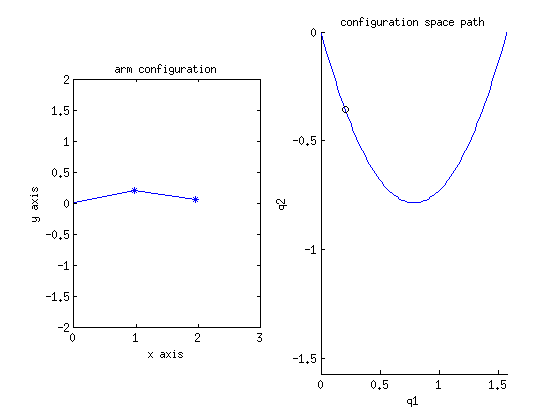
\includegraphics[width=0.8\textwidth]{pics/dynamic_singularity_pose}
\caption{Manipulator's $\mathbb{C}$-space path alongside the configuration of the end-effector at which there is unclear path-acceleration}
\label{fig:dynamic_singularity}
\end{figure}

\subsection{Bobrow's Algorithm}\label{sec:bobrow}

The implementation of this is the first milestone in the project. Starting with a 2-link manipulator and the dynamics model of the arm, initial attempts at constructing retimings like in the original paper were met with difficulties due to "dynamic singularities".

\begin{figure}[h]
\centering
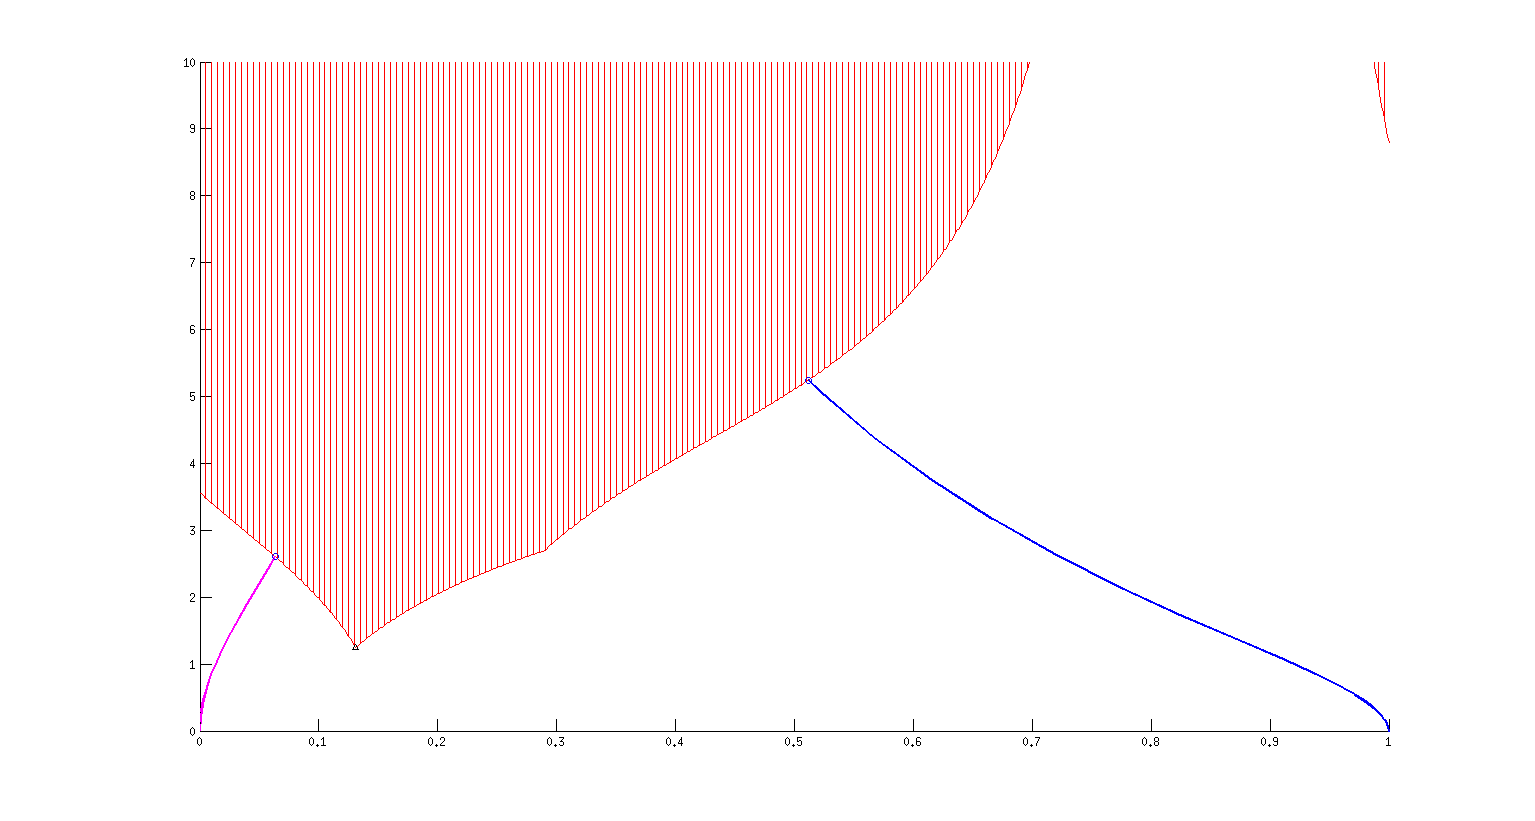
\includegraphics[width=0.8\textwidth]{pics/box_constraint_mvc}
\caption{Maximum Velocity curve in the $s$-$\dot{s}$ plane, with the $\beta$ and $\alpha$ acceleration profiles from start and end configurations.}
\label{fig:box_mvc}
\end{figure}

\begin{figure}[h!]
\centering
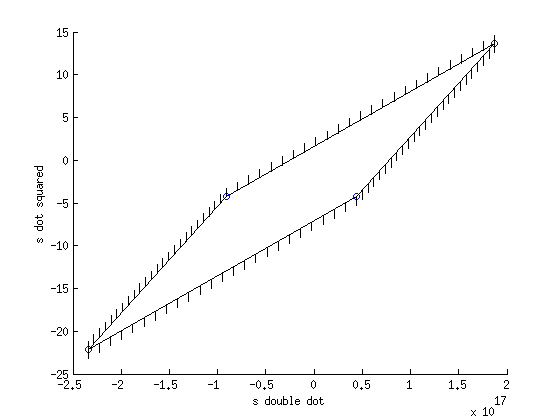
\includegraphics[width=0.8\textwidth]{pics/box_constraints_at_switch}
\caption{Constraints on $\dot{s}$ and $\ddot{s}$ at the irregular switch point. The exaggerated scale of the $\ddot{s}$ means a practically unbounded range of path accelerations can be chosen at the point of maximum path velocity $\dot{s}_{max}$}
\label{fig:box_constraints}
\end{figure} 

An example of this crops up at the manipulator configuration in the path described in Figure~\ref{fig:dynamic_singularity}. The retiming curve for this $\mathbb{C}$-space path is partially constructed in Figure~\ref{fig:box_mvc} with a switch-point that has ambiguous path acceleration limits. Figure~\ref{fig:box_constraints} shows the constraints on $\dot{s}$ and $\ddot{s}$ at the problematic point, which shows that at maximum path velocity, $\dot{s}_{max}$, there is an unbounded range of feasible path accelerations, $\ddot{s}$. This makes constructing the switching curve at this point ill-posed, since it runs counter to the expectation that at maximum path velocity there is a single feasible path acceleration at every other position along the path.

\begin{figure}[h!]
\centering
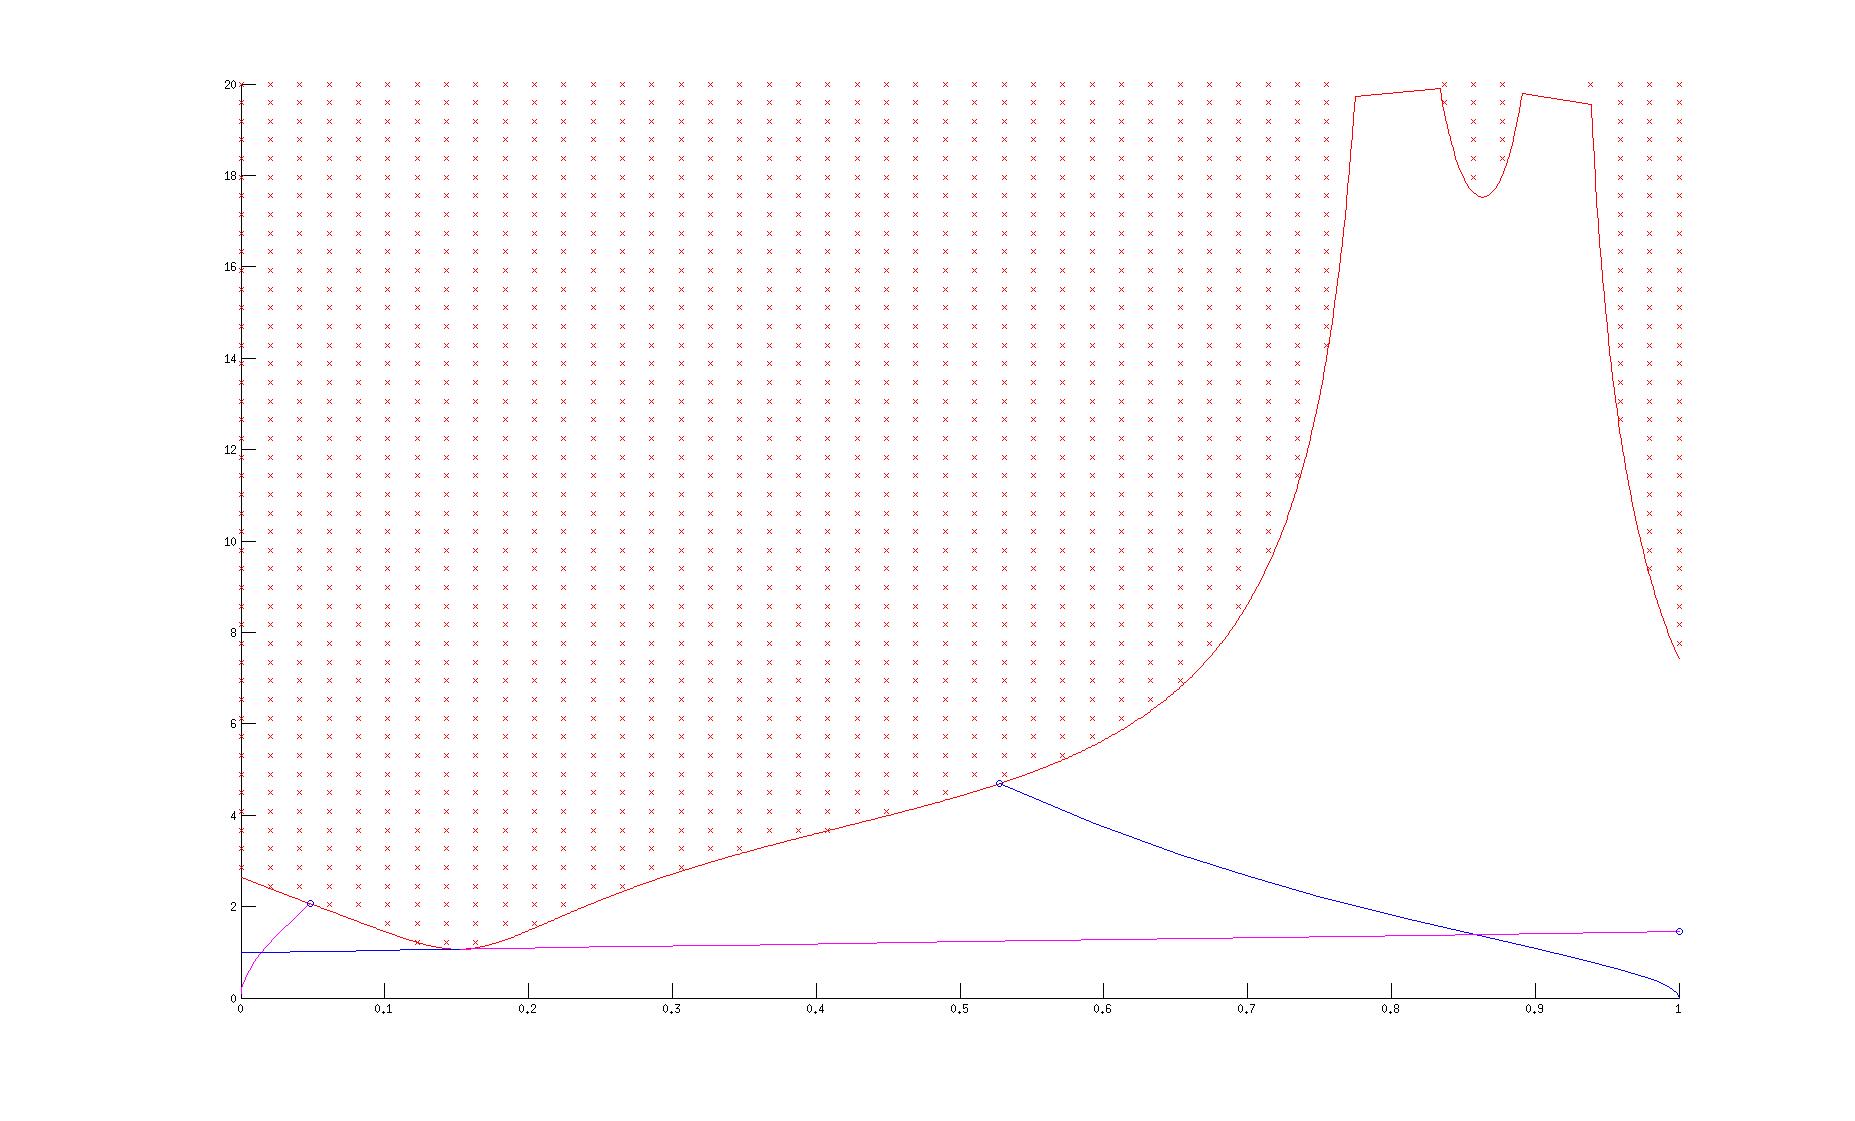
\includegraphics[width=0.8\textwidth]{pics/bobrow_path}
\caption{Demonstration of successful trajectory retiming curve constructed using elliptical torque contraints.}
\label{fig:elliptical}
\end{figure}

The problem can be circumvented with the insight that the problem arises due to box constraints on the torque. Using elliptical constraints~\cite{shiller1992computation}, the trajectory retiming curve can be constructed in the absence of such "singular" points. The results of this for the same manipulator path shown above are demonstrated in Figure~\ref{fig:elliptical}.

With the implementation of the basic retiming curve being constructed, it is now possible to explore strategies for dealing with dynamic obstacles in this domain.

\subsection{Moving Obstacles}\label{subsec:obs}

Dealing with moving obstacles may create inadmissible islands to retimings below the maximum-velocity curve of Bobrow's algorithm~\cite{shin1985minimum}. This isn't exactly accurate, and in order to represent moving obstacles in the framework for the retiming algorithm, a third dimension is added to the phase plane where the retiming is created. The third dimension is time, and it provides benefits to retiming in that the moving obstacle's representation can be simplified.

Given a path, a moving obstacle that intersections this path, one can construct an infeasible region for the phase-plane curve to pass through. Through use of this 3d construct, the hope is to be able to decide on time-optimal motions which result in collisions with the object. Obstacles can be represented as intervals in $s$ and $t$.

\ffig{pics/representation3d1}{}{rep3d1}
\ffig{pics/representation3d2}{}{rep3d2}
\ffig{pics/representation3d3}{}{rep3d3}
\ffig{pics/representation3d4}{}{rep3d4}

\subsection{Prototypical Successor Generation}\label{subsec:succ}

\ffig{pics/planner/initial_exp1}{}{iexp1}
\ffig{pics/planner/initial_exp2}{}{iexp2}
\ffig{pics/planner/second_exp1}{}{sexp1}
\ffig{pics/planner/second_exp2}{}{sexp2}
\ffig{pics/planner/second_exp5}{}{sexp5}
\ffig{pics/planner/second_exp4}{}{sexp4}
%------------------------------------------------

%------------------------------------------------

%----------------------------------------------------------------------------------------
%	BIBLIOGRAPHY
%----------------------------------------------------------------------------------------

\bibliographystyle{unsrt}

\bibliography{bibliography}

%----------------------------------------------------------------------------------------

\end{document}
